
%(BEGIN_QUESTION)
% Copyright 2007, Tony R. Kuphaldt, released under the Creative Commons Attribution License (v 1.0)
% This means you may do almost anything with this work of mine, so long as you give me proper credit

The following functional diagram documents a three-element boiler feedwater control system:

$$\includegraphics[width=15.5cm]{i01791x01.eps}$$

Identify all symbols in this diagram, explaining how they illustrate the control strategy of a three-element system.

\underbar{file i01791}
%(END_QUESTION)





%(BEGIN_ANSWER)

I'll let you research the meanings of functional diagram symbols.

%(END_ANSWER)





%(BEGIN_NOTES)

The ``A'' diamonds represent {\it adjustable} parameters, such as manual output or setpoint, while the ``T'' diamonds represent {\it transfer} (signal switching) blocks.

%INDEX% Documentation, functional: symbol identification
%INDEX% Documentation, functional: three-element boiler drum level control
%INDEX% Process: boiler feedwater control

%(END_NOTES)


